\chapter{Diagrama de classes}

\begin{flushright}
	\textit{
		Dedique-se aos estudos para que eles o façam \\
		melhor para a sociedade e para si mesmo.
	} \\
	
	\textbf{Alvaro Granha Loregian}
\end{flushright}

O modelo de caso de uso é formado por diversos elementos que tem como propósito o fornecimento de uma visão do ponto de vista externo ao sistema. Essa funcionalidade, externamente observada, é fornecida por meio da colaboração entre diversos elementos, os quais são chamados de \textbf{objetos}. A colaboração entre os objetos podem ser vista em dois aspectos, os \textbf{dinâmicos} e \textbf{os estruturais estáticos}.

O aspecto dinâmico diz respeito a forma com que os objetos realizam as trocas de mensagens e as reações a eventos que ocorrem no sistemas. Já os estruturais estáticos permite visualizar como o sistema está estruturado internamente para que as funcionalidades visíveis sem produzidas \cite{bezerra2016principios}.

Assim, realizaremos uma introdução aos aspectos estruturais estáticos, demostrando os elementos que o diagrama de classes utiliza para a representar um sistema orientado a objeto. O diagrama de classe, segundo \citeonline{guedes2018uml}, é um dos mais importante e mais utilizados diagramas da UML, o qual permite a visualização da \textbf{classes} que comporão o sistemas com seus respectivos \textbf{atributos}, \textbf{métodos} e pelo relacionamento entre estes.

\section{Modelo de classes}

A medida que o sistemas é desenvolvido, o modelo de classe pode evoluir para demostrar o sistema com maior riqueza de detalhes. Assim, podemos estudar três níveis de detalhamento: \textbf{domínio}, \textbf{especificação} é \textbf{implementação} \cite{bezerra2016principios}.

\begin{itemize}
	\item \textbf{Modelo de domínio: } Nesse modelo não é levado em consideração como o sistemas será implementado mas apenas as classes que o comporão.
	\item \textbf{Modelo de especificação: } Já no modelo de especificação são adicionados detalhes específicos relacionados a solução do software.
	\item \textbf{Modelo de implementação: } Esse modelo corresponde a implementação das classes em alguma linguagem de programação. 
\end{itemize}

\section{Diagrama de classes}

O diagrama de classes, como dito anteriormente, é um dos mais importantes para o desenvolvimento de um sistema orientado a objeto. 

Como todos os diagramas da UML, o diagrama de classe é composto de elementos que, consequentemente, possuem também suas responsabilidades. Assim, veremos todos este elementos, essenciais para o modelo de domíno, e como eles interagem entre si.

Lembre-se que, o conceito relacionado a cada um já foi apresentado no Capítulo \ref{cap:cap1}.

\subsection{Classes}

Uma classe é representada por meio de uma \textbf{caixa} com, no máximo, trés compartimentos. No compartimento superior é exibido o nome da classe, o qual é o único elemento obrigatório. 

No segundo compartimento são declarados os atributos. Este, como visto no \ref{cap:cap1}, armazenam os dados que um objeto armazena. Por fim, no último compartimento são declarados os métodos. 

Assim, segundo \citeonline{bezerra2016principios}, as possíveis anotações para que possamos representar uma classe utilizando as notações UML são representadas na Figura \ref{fig:notacoes-uml-diagrama-de-classes}.

\begin{figure}[H]
	\centering
	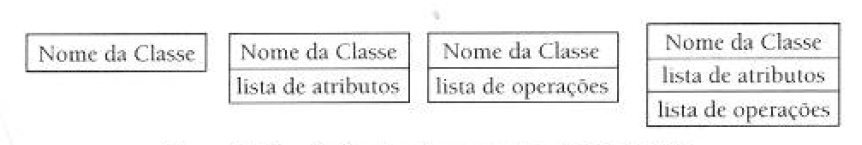
\includegraphics[scale=0.5]{imagens/notacoes-uml-classes.png}
	\caption{Possíveis notações para uma classe em UML.}
	\legend{Fonte: \cite{bezerra2016principios}}
	\label{fig:notacoes-uml-diagrama-de-classes}
\end{figure} 

Por convenção o nome das classe sempre será no singular e iniciará com letra maiúscula usando sempre o a forma de escrita conhecida como \textit{CamenCase}. Já os atributos e métodos sempre iniciarão com letra minúscula, mas também seguirão o padrão \textit{CamenCase}. Os métodos devem expressar uma ação que o objeto da classe sabe realizar. Vejamos um exemplo da classe \textbf{\textit{ContaBancaria}}.

\begin{figure}[H]
	\centering
	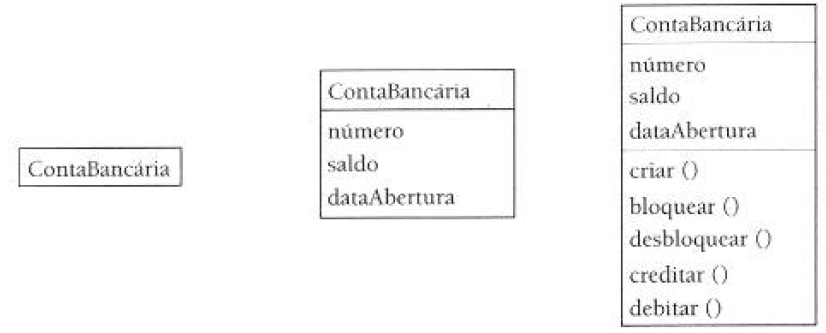
\includegraphics[scale=0.5]{imagens/exemplo-classe-conta-bancaria.png}
	\caption{Diferentes graus de detalhe para \textit{ContaBancaria}.}
	\legend{Fonte: \cite{bezerra2016principios}}
	\label{fig:exemplo-classe-conta-bancaria}
\end{figure}

\section{Exercícios de fixação}

Utilizando às notações aprendidas, identifique as possíveis classes, atributos e métodos para o problema abaixo.

\begin{enumerate}
	\item O professor \textbf{Picolo} precisa de um software para lhe ajudar a lembrar os aniversários de seus alunos. O software deve ser capaz de armazenar o nome do aluno, sua data de nascimento, seu e-mail, seu sexo e qualquer outro dado relevante. O software deve permitir o cadastro dos alunos, avisar quem faz aniversário no dia, calcular e mostrar a idade do aluno, exibir um relatório de aniversariantes no mês e outras funcionalidades que se julgar necessário.
	\item Faça o mesmo para o exercício 1 do exercício de fixação \ref{exer:001}
\end{enumerate}=